\documentclass{beamer}
\usetheme{greeniot}
\usepackage[utf8]{inputenc}
\usepackage{hyperref}
\usepackage{pgf}
\usepackage{tikz}
\usepackage{amsmath}
\usepackage{amsfonts}
\usepackage{amssymb}
\usepackage{graphicx}

\hypersetup{%
	pdftitle={Details of the ARM Architecture},
	pdfauthor={John Doe},
	pdfsubject={Sommerakademie der Studienstiftung, Leysin, 2016},
	pdfcreator=pdflatex,
	pdfproducer=pdflatex,
	pdfnewwindow=true,
	pdfpagemode=FullScreen,
	pdfview=FitBH,
	plainpages=false,
	baseurl={./}
}

% Title Page
\title[ARM Architecture]{%
	\Large Details of the ARM Architecture\\
	[5mm] \normalsize Sommerakademie in Leysin\\
	AG 2 -- Effizientes Rechnen
}
\author[John Doe]{John Doe}
\institute[]{%
	University of Awesomeness\\[3mm]
}
\date{August 2016}
\titlegraphic{%
	\vspace{5mm}%
	
\includegraphics[height=1.5cm]{logo_sdv.pdf}%
}

\begin{document}

%---------------------------------------------------------------------- SLIDE -
\begin{frame}
	\titlepage
\end{frame}

%---------------------------------------------------------------------- SLIDE -
\begin{frame}
	\frametitle{Outline}
	\tableofcontents
\end{frame}

%---------------------------------------------------------------------- SLIDE -
\section{Introduction}

% Show the table of contents again when a new section starts
%\AtBeginSection[]{%
%  \begin{frame}
%  \tableofcontents[currentsection]
%  \end{frame}
%}
\AtBeginSubsection[]{%
  \begin{frame}
  \tableofcontents[currentsubsection]
  \end{frame}
}

\begin{frame}[t]{Introduction}
  \begin{itemize}
    \item ARM is a RISC computer architecture / processor design
    \pause
    \item Developed by Advanced RISC Machines Ltd. (ARM), formerly Acorn, first released 1985
    \pause
    \item Licensing technology (IP) to semiconductor fabricators, NOT manufacturing themselves
    \pause
    \item Mainly used in \textbf{embedded systems}, e.g. mobile phones, tablets, ...
    \pause
    \item Advantages:
    \begin{itemize}
        \item Low power comsumption
        \item Price sensitive
        \item Flexibility
    \end{itemize}
    \pause
    \item As of 2014 50 billion ARM chips produced thus far, 15 bn in 2015\\ Share of about 90 \% at smartphones
  \end{itemize}
\end{frame}

%=========== TECHINCAL PART ===================%
\section{Technical Design}
\subsection{RISC vs. CISC}
\begin{frame}[t]{In General}
    \begin{itemize}
        \item<1-3,4->\textbf{RISC / CISC:} \textbf{R}educed \textbf{/ C}omplex \textbf{I}nstruction \textbf{S}et \textbf{C}omputing
        \item<2-3,4-> RISC: simple, but powerful instructions, executed in one cycle
        \item<2-3,4-> CISC: more and complex instructions, more work done in the core
        \item<3,4-> RISC architecture reduces hardware complexity and emphasizes software/compiler complexity 
    \end{itemize}
    \begin{alertblock}{Summary}<4->
    RISC reduces amount of hardware, CISC focuses performance
    \end{alertblock}
\end{frame}

\begin{frame}[t]{Major Design Rules of RISC}
    \begin{enumerate}
        \item<1-> \textbf{Instructions:} Only basic instructions, complicated operations synthesized by elementary instructions, fixed length
        \item<2-> \textbf{Pipelines:} Instructions always decoded in one pipeline stage, no need for microprograms
        \item<3-> \textbf{Registers:} Larger, general-purpose register set. Serves as fast memory store
        \item<4-> \textbf{Load/Store architecture:} Processor operates only on registers. Load and Store instructions access external memory
    \end{enumerate}
\end{frame}

%-------- INSTRUCTION SET ------------%
\subsection{Register Set}
\begin{frame}[t]{Registers}
    \begin{itemize}
        \item<1-> Total of 16 registers, each 32-bit in size
        \item<2-> Usually three dedicated registers: 
        \begin{itemize}
            \item r13 as stack pointer, designates stack memory frame
            \item r14 as link register, return address for subroutines
            \item r15 as program counter, address of next instruction
        \end{itemize}
        \item<3-> Additionally "Current Program Status Register" (CPSR)\\ 
    \end{itemize}
\end{frame}

\subsection{Instruction Set}

\begin{frame}[t]{ARM-specific Instruction Set Features}
  ARM Instruction Set differs from a strict RISC implementation:
  \begin{itemize}
      \item<1-> Load/Store multiple instructions have variable cycle length, higher code density, better performance by sequential memory access
      \item<2-> Conditional executions possible, reducing branches
      \item<3-> Inline barrel shifter
  \end{itemize}
  \uncover<4->{Supported instruction set modes:}
  \begin{itemize}
      \item<4-> Jazelle provides direct support of Java bytecode
      \item<4-> Thumb instructions
  \end{itemize}
\end{frame}

\begin{frame}[t]{Thumb Instructions}
    \begin{itemize}
        \item<1-> 16-Bit long instruction subset with most used instructions
        \item<2-> Enhances code density substantially, about 30 \% saving
        \item<2-> Important for embedded devices
        \item<3-> Lack of performance due to less functionality
    \end{itemize}
\end{frame}

\subsection{Evolution of the Pipeline}
\begin{frame}[t]{Basic Pipeline Scheme}
\begin{itemize}
    \item<1-> Up to ARM7 : Fetch - Decode - Execute
    \item<1-> With ARM9 : Fetch - Decode - Execute - \alert{Memory} - \alert{Write}
    \item<1-> With ARM10 : Fetch - \alert{Issue} -  Decode - Execute - Memory - Write
    \item<1-> Newer generations up to 14 stage pipeline (e.g. ARM Cortex-A8)
    \item<1-> ARM Cortex-A8 first to incorporate superscalar elements
\end{itemize}
\begin{center}
\uncover<2->{Classical distinction between RISC and CISC blurs the more it has been developing}
\end{center}

\end{frame}

%---------------------------------------------------------------------- SLIDE -

\section{Practical Issues}

\subsection{Power Consumption}
\begin{frame}[t]{Power Consumption: RISC Architecture}
    \begin{itemize}
        \item<1-> RISC architecture means processor design with less transistors
        \item<1-> $\Rightarrow$ Less switching activity and thus less power consumption!
    \end{itemize}
     
    \begin{tabular}{lll}
     \uncover<2->{Comparison: & ARM Cortex-A9 & Intel Core i7-960}\\
     \uncover<2->{& 26 Million Transistors & 731 Million Transistors}\\
     \uncover<3->{& 0.5 - 1.9 W & 130 W (TDP)}
    \end{tabular}

\end{frame}    

\begin{frame}[t]{Power Consumption: SoCs}
    \begin{itemize}
        \item<1-> ARM design allows purpose-oriented optimization
        \item<2-> \textbf{System-on-a-Chip} (SoC): Suitable additional components melted together with ARM core 
        \item<2-> Only required components $\Rightarrow$ Only required power
    \end{itemize}
\end{frame}

\subsection{Heat Dissipation}
\begin{frame}[t]{Heat Dissipation}
  \begin{itemize}
   \item<1-3> Due to low power consumption: heat dissipation generally lower
   \item<2-3> Hot spots can be problematic during longer computing times
   \item<2-3> Difficult to spread the heat in little cases
   \item<3> Liquid cooling/heat pipe technique in smartphones
  \end{itemize}
\end{frame}

\begin{frame}{Heat Dissipation}
\begin{figure}
 \centering
    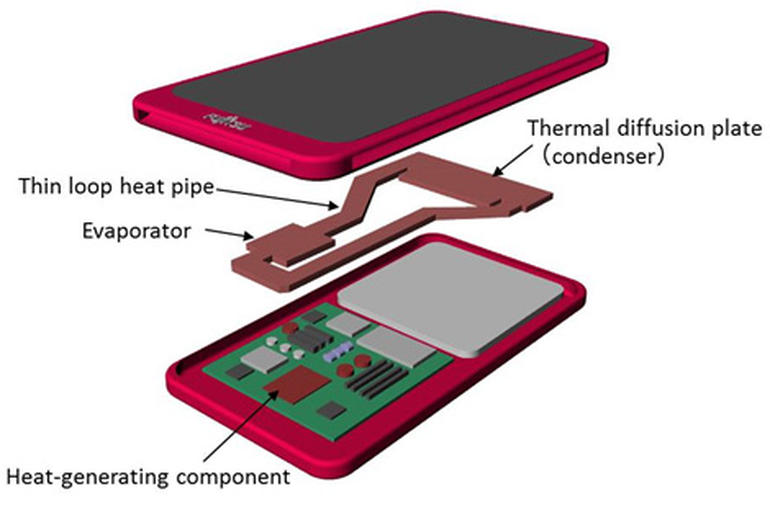
\includegraphics[width=0.8\textwidth]{cooling.jpg}
    \caption{\url{http://www.zdnet.com/article/fujitsu-has-a-cool-liquid-answer-to-hot-spots-in-smartphones/}}
\end{figure}
\end{frame}


\section{Markets and Success}

\begin{frame}[t]{The ARM Ecosystem}
    \begin{itemize}
        \item Licensing model allows various companies to implement technology
        \item SoCs for every conceivable purpose powered by ARM cores
        \item Creating versatile, specialized market based on a common architecture
        \item ARM instruction set already dominant on smartphone market (Android and iOS)
    \end{itemize}
\end{frame}

\begin{frame}{Applications of ARM}
\begin{figure}
    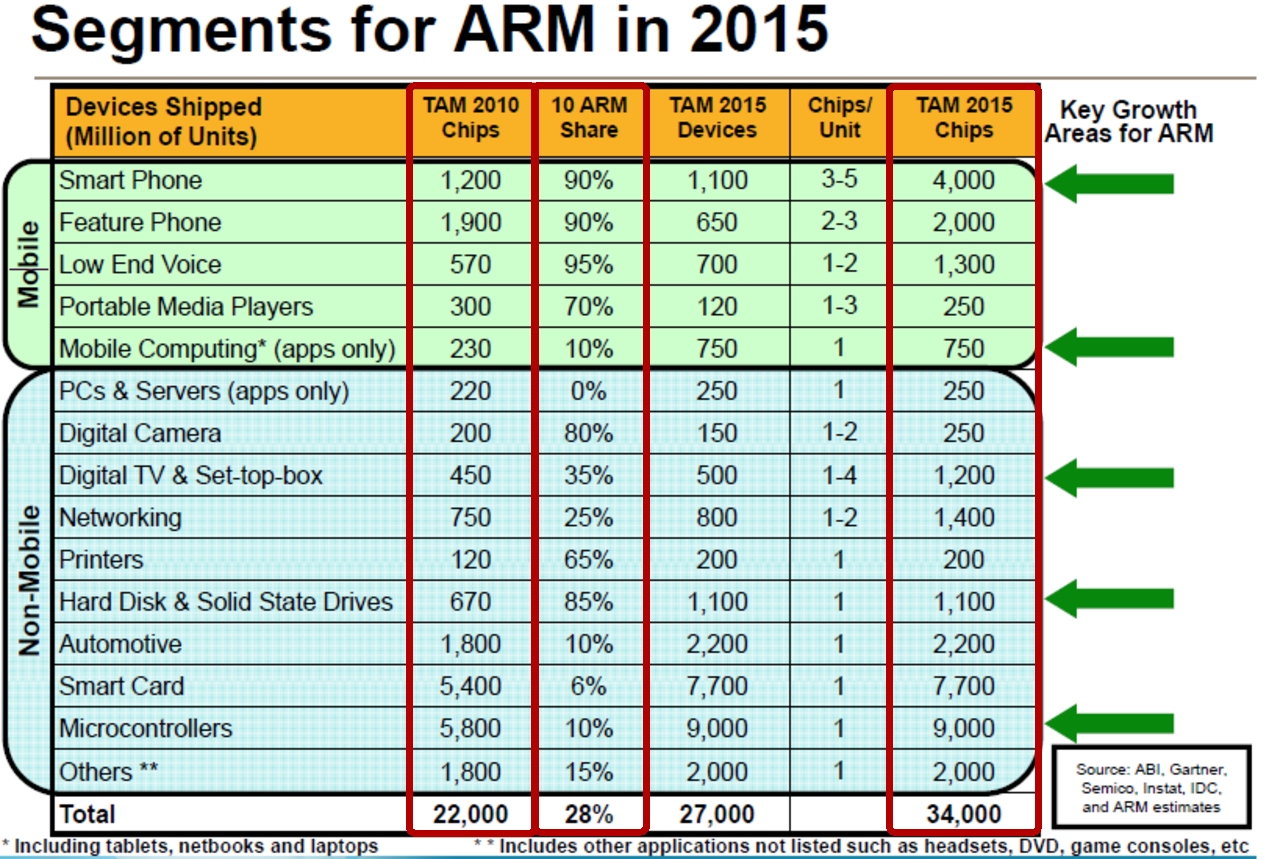
\includegraphics[width=0.75\textwidth]{arm2015_new.pdf}
    \caption{\url{http://www.cityindex.co.uk/market-analysis/market-news/40069092016/arm-shares-steady-on-firm-grip-of-smartphone-market/}}
\end{figure}
\end{frame}

\begin{frame}{Competition with PC Market}
 \begin{center}
 \begin{figure}
  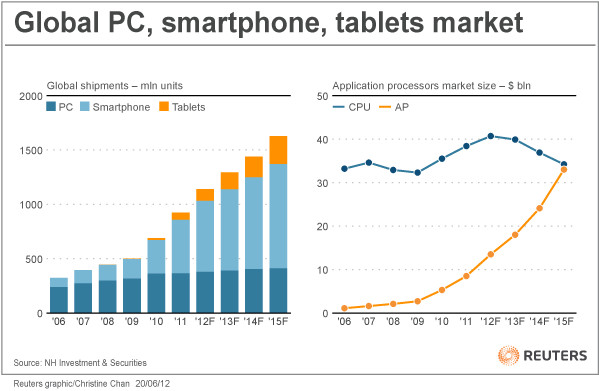
\includegraphics[width=0.8\textwidth]{procshare.jpg}
  \caption{\url{http://gadgets.ndtv.com/mobiles/news/smart-logic-samsung-chips-away-at-intel-lead-234639}}
 \end{figure}
\end{center}
\end{frame}


%\begin{frame}[t]{Applications of ARM}

%\begin{itemize}
% \item<1-> Vendors using ARM technology: Apple, Samsung, Texas Instruments, Qualcomm, Nvidia,...
% \item<2-> In 2015, 15 Billion ARM-based chips produced
%\end{itemize}
%\end{frame}

\section{Alternatives and Outlook}

\subsection{Further Developments in ARM}
\begin{frame}[t]{64-bit ARM Architecture}
 \begin{itemize}
  \item ARM Cortex-A50 series released in 2013 with 64-bit architecture
  \item First consumer device: iPhone 5S with Apple A7 processor
  \item Improvements:
  \begin{itemize}
    \item Using 64-bit adresses, no 3.5 GB memory limitation
    \item 31 instead of 15 general purpose registers
  \end{itemize}
\end{itemize}
\end{frame}

\begin{frame}[t]{Future Markets}
    \begin{figure}
    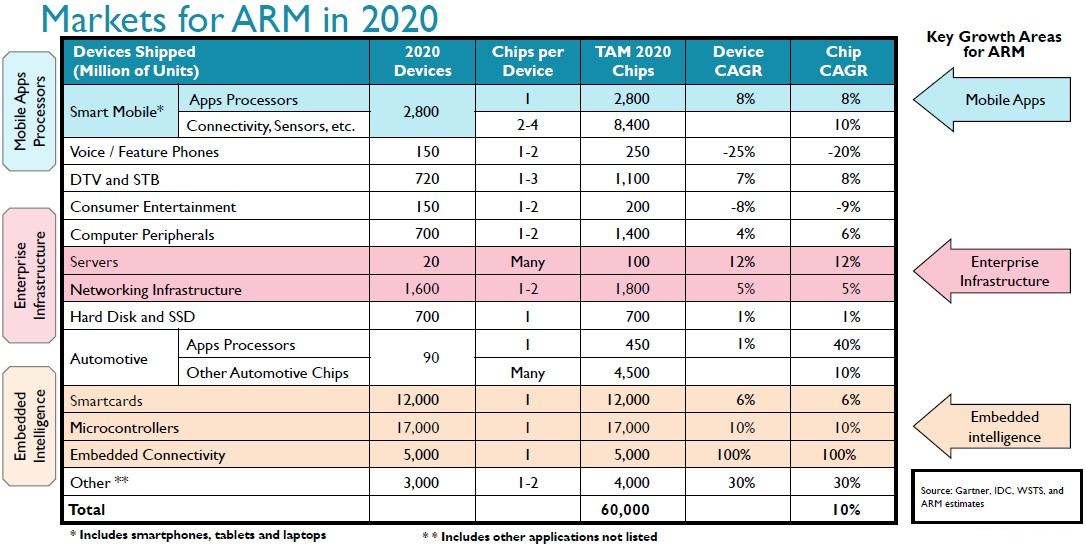
\includegraphics[width=\textwidth]{arm2020.jpg}
    \caption{\url{http://www.nextplatform.com/2015/10/06/why-are-we-still-waiting-for-arm-servers/}}
    \end{figure}
\end{frame}

\subsection{Mill Architecture}
\begin{frame}[t]{Mill Architecture}
\uncover<3>{\begin{figure}
 \centering
  \includegraphics<3>[width=0.35\textwidth]{add_belt.png}
  \caption{\url{http://millcomputing.com/blog/wp-content/uploads/2014/02/intro_belt.png}}
\end{figure}}
\begin{itemize}
 \item<1,2,4-> Radical new approach to processor design
 \item<2,4-> Key concept: Register Belt instead of random access registers
 \item<2,4-> Shall improve performance by less register accesses
\end{itemize}
\uncover<4->{\alert{Problems:}}
\begin{itemize}
 \item<4-> Very, very, complex programming
\end{itemize}

\end{frame}


\begin{frame}
  \begin{center}

   \texttt{<insert obligatory cookie/potato meme here>}

    \vspace{1cm}
    {\huge\bfseries Sänk ju!}
  \end{center}
\end{frame}

\end{document}
